\documentclass[10pt,a4paper]{article}
\usepackage[brazilian]{babel}
\usepackage[utf8x]{inputenc}
\usepackage[T1]{fontenc}
\usepackage{amsmath}
\usepackage{graphicx}
\usepackage[a4paper,left=3cm,right=2cm,top=2.5cm,bottom=2.5cm]{geometry}

\usepackage{listings}
\usepackage{color}

\definecolor{dkgreen}{rgb}{0,0.6,0}
\definecolor{gray}{rgb}{0.5,0.5,0.5}
\definecolor{mauve}{rgb}{0.58,0,0.82}

\usepackage{hyperref}

\lstset{frame=tb,
  language=c,
  aboveskip=3mm,
  belowskip=3mm,
  showstringspaces=false,
  columns=flexible,
  basicstyle={\small\ttfamily},
  numbers=none,
  numberstyle=\tiny\color{gray},
  keywordstyle=\color{blue},
  commentstyle=\color{dkgreen},
  stringstyle=\color{mauve},
  breaklines=true,
  breakatwhitespace=true
  tabsize=3
}

\title{Relatório: Exercício Programa 01}
\author{Lucas Sung Jun Hong  (n.USP: 8124329)}
\begin{document}
\newpage
\maketitle
\newpage

\newpage
\tableofcontents
\newpage
\section{Estruturação do Programa}
	\subsection{Inserindo n a um vetor}
		\paragraph*{} Recebido {\bf n}, um {\tt unsigned long long int}, cada algarismo é inserido dentro de um vetor {\bf nArray[ ]}. Seu tamanho será {\bf x}, tal que {\bf x} foi obtido pela função {\tt int algCount}:
		\begin{lstlisting}
int algCount (unsigned long long int n) {
    int count = 0;

    while (n != 0) {
        n /= 10;
        count++;
    }
    return count;
}
		\end{lstlisting}

		\paragraph*{} O vetor contém na posição 0, o algarismo menos significativo e na posição x - 1, o algarismo mais significativo. Por exemplo:
		\paragraph*{} {\tt input: n = 65;  output: 5 6}

	\subsection{Circular Doubly Linked-List}
		\paragraph*{} Considerando que precisamos de números extremamente grandes, porém unidimensionais, pois trata-se de números elevados à uma potência de 2, foi optado uma lista circular duplamente encadeada. Desconhecemos o tamanho que necessitamos gerar a cada vez que um número é multiplicado por 2 e mais,precisamos atualizar os elementos constantemente. Assim, usando uma lista circular duplamente encadeada  facilita aumentar  algarismos extras sendo que só é preciso criar uma célula extra.
		\paragraph*{} No entanto, o problema de usar uma lista encadeada é "memory overhead" pois cada célula aponta duplamente para frente e para trás.
		\paragraph*{} A lista é criada da seguinte forma:
		\begin{lstlisting}
ListaCelula *crieListaCelula () {
    ListaCelula *lst;
    Celula *p;

    lst = malloc(sizeof(*lst));
    lst->head = malloc(sizeof(*lst->head));

    p = crieCelula();
    p->element = 2;

    lst->head->prox = p;
    lst->head->ant = p;
    p->prox = lst->head;
    p->ant = lst->head;

    return lst;
}
		\end{lstlisting}
		Ilustrativamente, a função faz o seguinte:
		
		\begin{figure}[h!]
		  \centering
		    
\includegraphics[scale=0.2]{01.jpg}
		  \caption{criação de uma lista}
		\end{figure}
		
		\paragraph*{} Ao dobrarmos o conteúdo de uma célula, obtemos um momento em que seu valor é maior que 9, ou melhor, teremos 2 algarismos (por exemplo o 18) dentro dessa célula. Nesse momento criamos uma nova célula e inserimos nela o algarismo mais significativo, deixando o algarismo menos significativo na céula inicial.
		\paragraph*{} A implementação no programa foi escrita de uma forma tal que a cada criação de uma nova célula, o dígito 1 já vem incluso, sendo apenas necessário obter o resto da divisão do número (maior que 9) por 10 e substituí-la na célula inicial.
		
		\begin{figure}[h!]
			\centering
				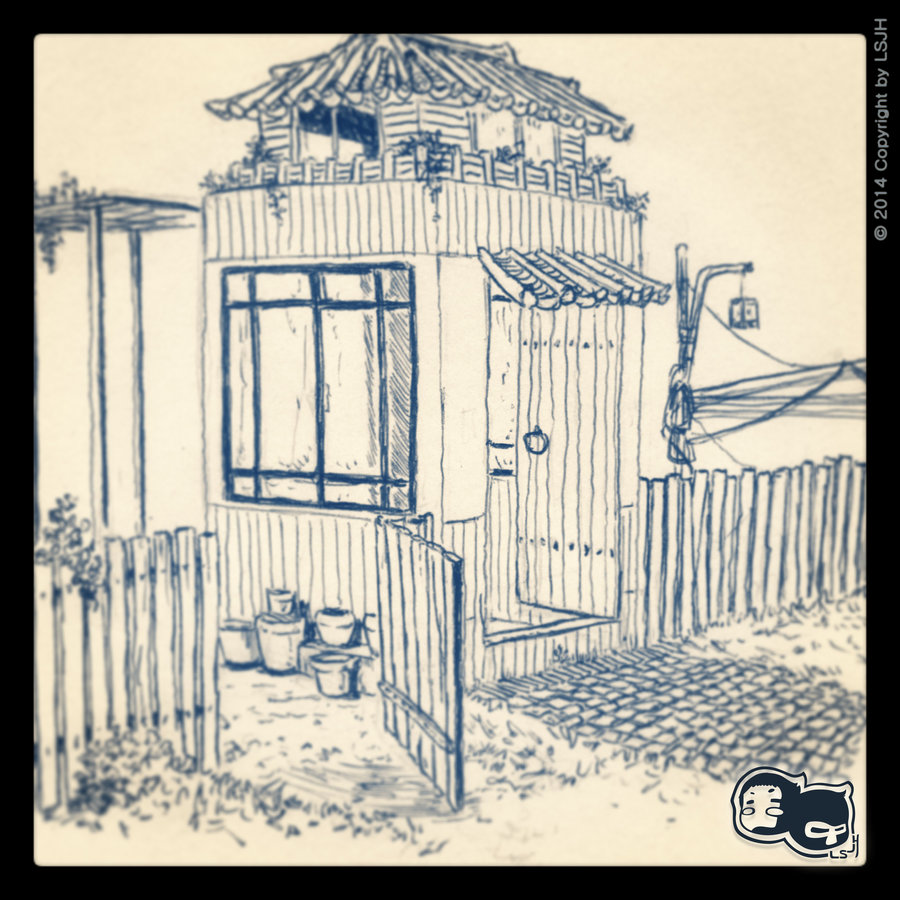
\includegraphics[scale=0.2]{02.jpg}
				\caption{Após de dobrar os algarismos, checamos de trás para frente para verificar se cada célula possui número > 9. Caso sim, atualizamos cada célula com a soma correta.}
		\end{figure}
		
\section{Quando comparamos?}
	\subsection{O que é $2^{min}$?}
	\paragraph*{} Temos $n$ com 0 $ \leq n  \leq 2*10^9$. Com $n$, podemos contar quantos algarismos contém em $n$, sendo esse valor: $x$. Assim, um número mínimo que contenha o $n$ é o seguinte: $n*10^{x + mod}$, tal que $mod = 1, 2, 3, ...$. Calculando o logaritmo na base 2 desse número podemos obter a potência desejada, tal que, 2 elevado à esse número contenha $n$. 
	\paragraph*{} Por exemplo: seja $n = 12$ então $x = 2$, com $mod = 1$. Então o número mínimo será 12000. assim:\\{\it (com mod = 1)}
		\begin{equation*}
		log_2 12000 = log_2 12*10^{2+1} =  log_2 12*10^3 = 
		\end{equation*}	
		\begin{equation*}
		log_2 12 + 3*(log_2 10) = 13.550
		\end{equation*}
	\\ como $min = $ $\lceil$ $(log_2(n) + ( (x + mod) * log_2(10) ))$ $\rceil$
		\begin{equation*}
		min = \lceil log_2 12000 \rceil = \lceil 13.550 \rceil = 14
		\end{equation*}
		
	\paragraph*{} Assim $2^{14}$ será o valor estimado. Em outras palavras, esperamos que $2^{14}$ seja o valor ideal que contenha os dígitos "12" no início. Mas $2^{14} = 16384$, portanto $12000$ não foi um bom valor. Aumentamos o $mod + 1$, portanto $mod = 2$, assim teremos: $x + (mod) = 2 + (2) = 4$, ou seja, aumentamos de 12,000 para 120,000.\\{\it (com mod = 2)}
	\begin{equation*}
	log_2 120000 = log_2 12 * 10^{2+2} =  log_2 12 * 10^4 
	\end{equation*}	 
	\paragraph*{} E assim aumentamos $mod + 1$ caso $2^{min}$ não for o valor esperado até encontrarmos o valor ideal.
	
	\subsection{Comparando $2^{pot}$ com $2^{min}$}
		\paragraph*{} O programa calcula $2^{pot}$, com $pot = 1, 2, 3, ...$. No momento em que $pot = min$, chama-se a função {\tt compara(lst, nArray, x)}, que compara $2^{pot}$ com $2^{min}$. Caso $2^{min} \neq 2^{pot}$, aumentamos o valor de $min$ até encontrarmos o valor ideal.
\section{Maior valor testado}
	\subsection{13,7 minutos}
		\paragraph*{} O maior valor de n testado foi: 1,999,987,841.
		\paragraph*{} Sua saída foi: 904,665.
		\paragraph*{} Para tal n, o programa levou 825,97 segundos (13,7 minutos).
		\paragraph*{} O número calculado foi:
\newpage
\section{Bibliografia}
	\begin{itemize}
		\item \url{http://en.wikipedia.org/wiki/Power_of_two}
		\item \url{http://en.wikipedia.org/wiki/Binary_numeral_system}
		\item \url{http://en.wikipedia.org/wiki/Benford's_law}
		\item \url{http://en.wikipedia.org/wiki/Exponentiation}
		\item \url{http://en.wikipedia.org/wiki/Logarithm}
		\item \url{http://oeis.org/A001146}
		\item \url{http://en.wikibooks.org/wiki/LaTeX/}
		\item \url{http://stackoverflow.com/}
		\item \url{http://en.wikipedia.org/wiki/Bignum}
		\item \url{http://www.cs.utexas.edu/users/djimenez/utsa/cs1723/lecture1.html}
		\item \url{https://gmplib.org/}
		\item \url{https://www.khanacademy.org/math/algebra2/logarithms-tutorial/logarithmic-scale-patterns/v/benford-s-law-explanation--sequel-to-mysteries-of-benford-s-law}
		\item \url{http://valgrind.org/docs/manual/mc-manual.html}
		\item \url{http://valgrind.org/docs/manual/manual-core.html#opt.read-var-info}
		\item \url{http://valgrind.org/docs/manual/manual-core-adv.html#manual-core-adv.gdbserver-simple}
	\end{itemize}
\newpage
\end{document}